\chapter{THỰC NGHIỆM}
\label{chap:thucnghiem}

\section{Thiết lập}

\paragraph{Thuật toán và tham số.} Mọi lần chạy dùng \code{src/nsga2.py} của nhóm sau khi ghép nhánh
chính, với cấu hình mặc định: $N_{pop} = 80$, $G = 200$, lai ghép OX với $p_c = 0{,}7$, đột biến chuẩn
với $p_m = 0{,}1$ (Solomon) hoặc $0{,}2$ (case29), giải đấu kích thước 2, loại cá thể trùng, cắt tuyến
\code{capacity\_time}, tính hài lòng theo giờ đến. Các cải tiến của TV3 và TV4 đều tắt. Hai cải tiến của
TV2 dùng tham số mặc định nêu ở Chương~\ref{chap:init} và Chương~\ref{chap:ls}.

\paragraph{Instance.} C102-25, R201-50, RC201-100 và case29-29, đại diện cho ba kiểu phân bố khách của
bộ Solomon, ba cỡ bài toán và dữ liệu thực tế.

\paragraph{Cấu hình so sánh.}
\begin{itemize}
  \item \textbf{Gốc}: thuật toán của TV1, mọi cờ tắt.
  \item \textbf{init\_smart}: chỉ bật khởi tạo thông minh.
  \item \textbf{LS (reject)}: chỉ bật tìm kiếm cục bộ, chính sách lệch biên mặc định.
  \item \textbf{LS (evaluate\_actual)}: chỉ bật tìm kiếm cục bộ, chính sách \code{evaluate\_actual}.
  \item \textbf{init + LS}: bật cả hai, với từng chính sách lệch biên.
  \item \textbf{Gốc, cùng số lần đánh giá}: thuật toán gốc chạy thêm thế hệ để tổng số lần đánh giá bằng
        trung bình của cấu hình init + LS (evaluate\_actual) trên cùng instance (670, 1016, 1374 và 1030
        thế hệ cho bốn instance).
\end{itemize}
Cấu hình cuối cần thiết vì tìm kiếm cục bộ gọi bộ đánh giá nhiều hơn hẳn. So ở cùng 200 thế hệ là có lợi
cho các cấu hình có tìm kiếm cục bộ; so với thuật toán gốc được cấp cùng số lần đánh giá mới cho biết
tìm kiếm cục bộ có dùng ngân sách đánh giá hiệu quả hơn việc chạy thêm thế hệ hay không.

\paragraph{Seed.} Tinh chỉnh tham số dùng seed 100 đến 104. Kết quả báo cáo dùng seed 0 đến 9, giống
nhau cho mọi cấu hình. Không có tham số nào được chọn dựa trên seed 0 đến 9.

\paragraph{Chỉ số.} HV, IGD, SP và số điểm trên front tính bằng \code{src.runner analyze} của nhóm,
theo quy ước ở mục 2.7: tập tham chiếu và cận chuẩn hoá lấy chung từ mọi cấu hình, mọi seed trên cùng
instance. Giá trị $p$ là kiểm định Wilcoxon rank-sum trên 10 giá trị HV của cấu hình đó so với thuật toán
gốc 200 thế hệ. Toàn bộ số liệu trong các bảng dưới đây được sinh tự động bởi
\code{scripts/tv2\_report\_figures.py}.

\section{Tinh chỉnh tham số}

Bảng~\ref{tab:tune} so ba tỉ lệ khởi tạo và bốn biến thể tìm kiếm cục bộ, mỗi biến thể thay đúng một
tham số so với mặc định, chạy trên seed 100 đến 104.

\begin{table}[H]
\centering
\caption{HV trung bình $\pm$ độ lệch chuẩn khi tinh chỉnh (seed 100--104; in đậm là biến thể tốt nhất
trong nhóm khởi tạo và nhóm tìm kiếm cục bộ)}
\label{tab:tune}
\resizebox{\textwidth}{!}{\begin{tabular}{@{}lllll@{}}
\toprule
Biến thể & C102-25 & R201-50 & RC201-100 & case29-29 \\
\midrule
Gốc & 0{,}682 $\pm$ 0{,}190 & 0{,}567 $\pm$ 0{,}134 & 0{,}362 $\pm$ 0{,}055 & 0{,}727 $\pm$ 0{,}109 \\
\midrule
init 20/20/60 & \textbf{1{,}216 $\pm$ 0{,}067} & \textbf{1{,}008 $\pm$ 0{,}115} & \textbf{1{,}007 $\pm$ 0{,}143} & 0{,}925 $\pm$ 0{,}082 \\
init 10/10/80 & 1{,}146 $\pm$ 0{,}085 & 0{,}959 $\pm$ 0{,}074 & 0{,}960 $\pm$ 0{,}087 & 0{,}892 $\pm$ 0{,}136 \\
init 30/30/40 & 1{,}170 $\pm$ 0{,}045 & 0{,}883 $\pm$ 0{,}155 & 1{,}002 $\pm$ 0{,}104 & \textbf{1{,}034 $\pm$ 0{,}111} \\
\midrule
LS reject & \textbf{0{,}801 $\pm$ 0{,}109} & 0{,}496 $\pm$ 0{,}100 & 0{,}380 $\pm$ 0{,}061 & 0{,}798 $\pm$ 0{,}168 \\
LS (evaluate\_actual) & 0{,}662 $\pm$ 0{,}160 & \textbf{0{,}698 $\pm$ 0{,}156} & \textbf{0{,}537 $\pm$ 0{,}068} & 0{,}798 $\pm$ 0{,}101 \\
LS pareto & 0{,}653 $\pm$ 0{,}188 & 0{,}591 $\pm$ 0{,}106 & 0{,}436 $\pm$ 0{,}072 & 0{,}668 $\pm$ 0{,}173 \\
LS $p_{ls}=0{,}1$ & 0{,}519 $\pm$ 0{,}316 & 0{,}610 $\pm$ 0{,}157 & 0{,}431 $\pm$ 0{,}080 & \textbf{0{,}812 $\pm$ 0{,}171} \\
\bottomrule
\end{tabular}
}
\end{table}

Tỉ lệ $0{,}2/0{,}2/0{,}6$ cho HV cao nhất trên ba trong bốn instance; trên case29, tỉ lệ $0{,}3/0{,}3/0{,}4$
tốt hơn. Vì không có tỉ lệ nào thắng đều, nhóm giữ tỉ lệ mặc định. Với tìm kiếm cục bộ, chính sách
\code{evaluate\_actual} tốt nhất trên R201-50 và RC201-100, \code{reject} tốt nhất trên C102-25. Trên
case29, hai chính sách bằng nhau (0,798) và giảm $p_{ls}$ xuống $0{,}1$ cho HV cao nhất (0,812).
Chấp nhận theo trội Pareto và giảm $p_{ls}$ không tốt hơn mặc định một cách nhất quán trên cả bốn
instance. Vì hai chính sách lệch biên cho kết quả trái chiều, thí nghiệm chính
chạy cả hai.

\section{Hiệu quả của khởi tạo thông minh}

\subsection{Quần thể ban đầu}

Bảng~\ref{tab:init} so quần thể ban đầu của thuật toán gốc và của \code{init\_smart} với cùng seed. HV ở
đây được chuẩn hoá theo hợp các front ban đầu của hai cấu hình, vì front ban đầu nằm ngoài vùng chuẩn
hoá của các front cuối.

\begin{table}[H]
\centering
\caption{Quần thể ban đầu (trung bình 10 seed): HV, $f_1$ nhỏ nhất và $f_3$ lớn nhất}
\label{tab:init}
\resizebox{\textwidth}{!}{\begin{tabular}{@{}lrrrrrr@{}}
\toprule
 & \multicolumn{3}{c}{Khởi tạo ngẫu nhiên (gốc)} & \multicolumn{3}{c}{init\_smart} \\
\cmidrule(lr){2-4}\cmidrule(l){5-7}
Instance & HV & $f_1$ nhỏ nhất & $f_3$ lớn nhất & HV & $f_1$ nhỏ nhất & $f_3$ lớn nhất \\
\midrule
C102-25 & 0{,}120 $\pm$ 0{,}024 & 3.804{,}4 & 0{,}561 & 1{,}090 $\pm$ 0{,}118 & 2.424{,}1 & 0{,}718 \\
R201-50 & 0{,}084 $\pm$ 0{,}022 & 11.145{,}8 & 0{,}376 & 0{,}641 $\pm$ 0{,}039 & 9.391{,}8 & 0{,}704 \\
RC201-100 & 0{,}067 $\pm$ 0{,}013 & 45.377{,}4 & 0{,}259 & 0{,}639 $\pm$ 0{,}030 & 24.106{,}6 & 0{,}496 \\
case29-29 & 0{,}257 $\pm$ 0{,}050 & 2.919{,}9 & 0{,}793 & 1{,}102 $\pm$ 0{,}010 & 2.570{,}3 & 0{,}828 \\
\bottomrule
\end{tabular}
}
\end{table}

Trên cả bốn instance, quần thể ban đầu của \code{init\_smart} có HV gấp khoảng 4 đến 10 lần, chi phí nhỏ nhất
thấp hơn và mức hài lòng lớn nhất cao hơn. Khác biệt lớn nhất ở RC201-100: chi phí nhỏ nhất giảm từ
45.377 xuống 24.107 CNY, mức hài lòng lớn nhất tăng từ 0,259 lên 0,496. Hình~\ref{fig:init} cho thấy
nguyên nhân: các cá thể dựng từ thứ tự NN nằm ở vùng chi phí thấp, các cá thể dựng từ thứ tự TW nằm ở
vùng hài lòng cao, còn các cá thể ngẫu nhiên (của cả hai cấu hình) nằm chung một đám ở vùng kém.

\begin{figure}[H]
\centering
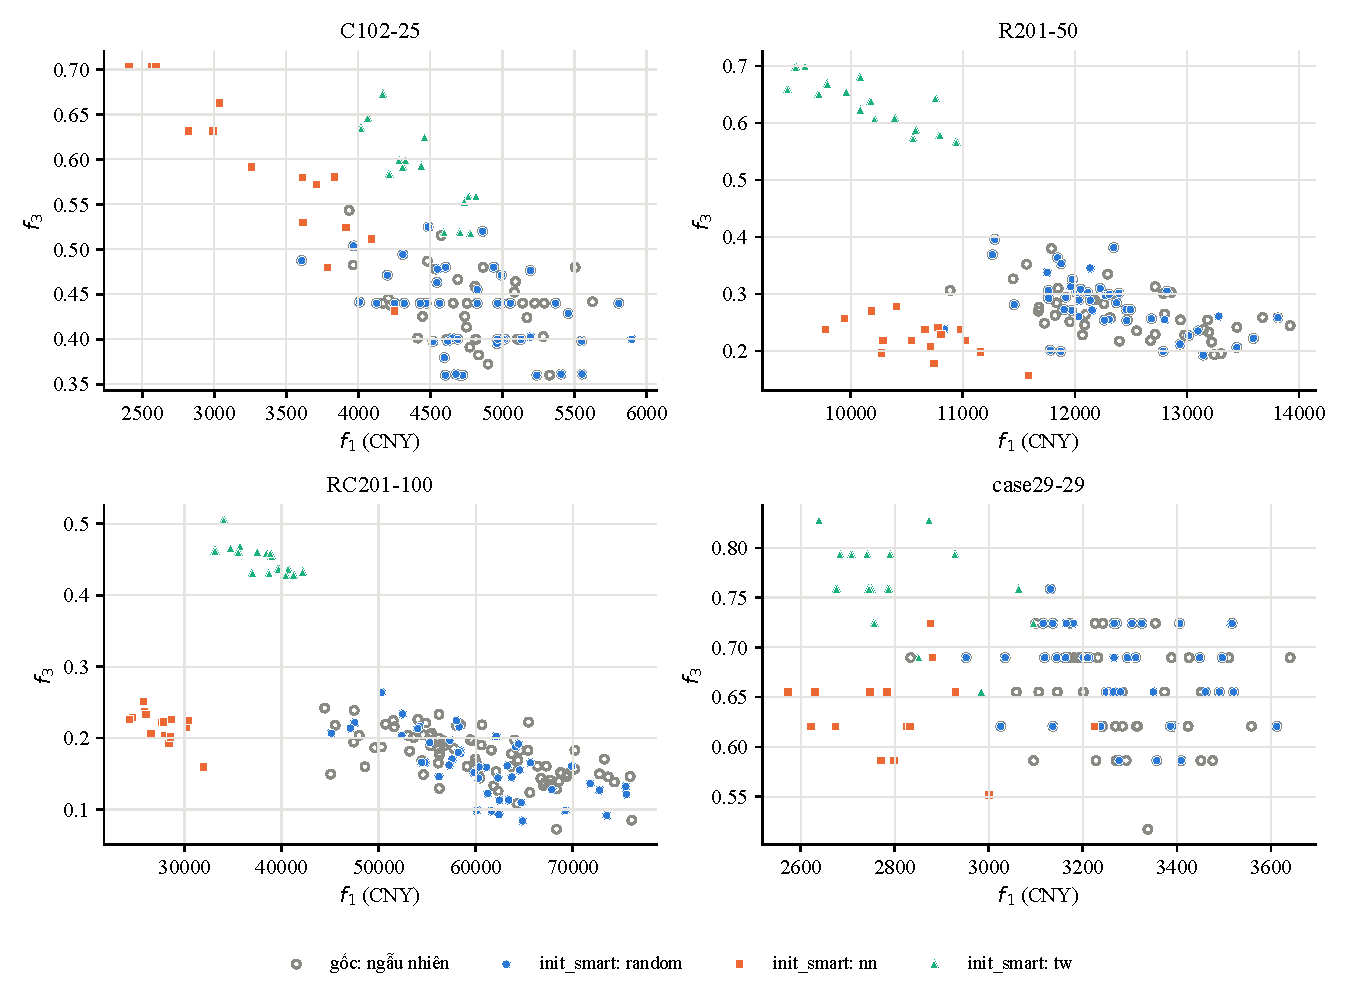
\includegraphics[width=\textwidth]{quan_the_dau.pdf}
\caption{Quần thể ban đầu với seed 0 trên mặt phẳng $f_1$--$f_3$: thuật toán gốc (vòng tròn rỗng) và
\code{init\_smart} theo từng nguồn}
\label{fig:init}
\end{figure}

\subsection{Kết quả cuối}

Ở cùng 200 thế hệ và cùng 16.080 lần đánh giá, \code{init\_smart} cho HV cao hơn hẳn thuật toán gốc trên
cả bốn instance với $p < 0{,}001$ (bảng~\ref{tab:main-c102} đến~\ref{tab:main-case29}): C102-25 từ 0,663
lên 1,099; R201-50 từ 0,385 lên 0,687; RC201-100 từ 0,328 lên 0,877; case29-29 từ 0,550 lên 0,775. IGD
giảm tương ứng và độ lệch chuẩn của HV nhỏ hơn, tức kết quả ổn định hơn giữa các seed. Cải tiến này
không tốn thêm lần đánh giá nào và thời gian chạy gần như không đổi.

So với thuật toán gốc được chạy dài hơn 3,3 đến 6,8 lần số lần đánh giá, \code{init\_smart} 200 thế hệ
vẫn tốt hơn trên C102-25 (1,099 so với 0,911, $p = 0{,}034$) nhưng kém hơn trên ba instance còn lại
($p$ từ 0,0007 đến 0,028). Như vậy khởi tạo thông minh chủ yếu giúp thuật toán tới vùng tốt nhanh hơn;
khi được chạy đủ lâu, thuật toán gốc vẫn bắt kịp và vượt.

\section{Hiệu quả của tìm kiếm cục bộ}

\subsection{Bảng kết quả}

\begin{table}[H]
\centering
\caption{Kết quả trên C102-25 (10 seed; $G$ là số thế hệ; $p$ so với Gốc 200 thế hệ)}
\label{tab:main-c102}
\resizebox{\textwidth}{!}{\begin{tabular}{@{}lrllrrrrr@{}}
\toprule
Cấu hình & $G$ & HV & IGD & SP & Số điểm & Số lần đánh giá & Thời gian (s) & $p$ \\
\midrule
Gốc & 200 & 0{,}663 $\pm$ 0{,}248 & 0{,}366 $\pm$ 0{,}112 & 0{,}072 & 9{,}7 & 16.080 & 6{,}3 & -- \\
Gốc, cùng số lần đánh giá & 670 & 0{,}911 $\pm$ 0{,}208 & 0{,}274 $\pm$ 0{,}045 & 0{,}037 & 21{,}1 & 53.680 & 18{,}9 & 0{,}019 \\
init\_smart & 200 & 1{,}099 $\pm$ 0{,}097 & 0{,}239 $\pm$ 0{,}028 & 0{,}045 & 16{,}7 & 16.080 & 5{,}1 & $<$0{,}001 \\
LS (reject) & 200 & 0{,}596 $\pm$ 0{,}229 & 0{,}396 $\pm$ 0{,}178 & 0{,}044 & 15{,}3 & 65.719 & 23{,}8 & 0{,}705 \\
LS (evaluate\_actual) & 200 & 0{,}691 $\pm$ 0{,}137 & 0{,}346 $\pm$ 0{,}074 & 0{,}089 & 13{,}8 & 56.704 & 20{,}9 & 0{,}545 \\
init + LS (reject) & 200 & 1{,}177 $\pm$ 0{,}076 & 0{,}235 $\pm$ 0{,}064 & 0{,}103 & 6{,}3 & 57.251 & 19{,}8 & $<$0{,}001 \\
init + LS (evaluate\_actual) & 200 & \textbf{1{,}193 $\pm$ 0{,}067} & \textbf{0{,}210 $\pm$ 0{,}018} & 0{,}098 & 6{,}9 & 53.661 & 19{,}1 & $<$0{,}001 \\
\bottomrule
\end{tabular}
}
\end{table}

\begin{table}[H]
\centering
\caption{Kết quả trên R201-50}
\label{tab:main-r201}
\resizebox{\textwidth}{!}{\begin{tabular}{@{}lrllrrrrr@{}}
\toprule
Cấu hình & $G$ & HV & IGD & SP & Số điểm & Số lần đánh giá & Thời gian (s) & $p$ \\
\midrule
Gốc & 200 & 0{,}385 $\pm$ 0{,}080 & 0{,}448 $\pm$ 0{,}083 & 0{,}030 & 19{,}7 & 16.080 & 10{,}8 & -- \\
Gốc, cùng số lần đánh giá & 1016 & \textbf{0{,}898 $\pm$ 0{,}107} & \textbf{0{,}110 $\pm$ 0{,}048} & 0{,}012 & 48{,}3 & 81.360 & 47{,}0 & $<$0{,}001 \\
init\_smart & 200 & 0{,}687 $\pm$ 0{,}074 & 0{,}212 $\pm$ 0{,}047 & 0{,}026 & 25{,}9 & 16.080 & 10{,}7 & $<$0{,}001 \\
LS (reject) & 200 & 0{,}420 $\pm$ 0{,}105 & 0{,}414 $\pm$ 0{,}108 & 0{,}022 & 33{,}3 & 113.295 & 71{,}1 & 0{,}545 \\
LS (evaluate\_actual) & 200 & 0{,}505 $\pm$ 0{,}108 & 0{,}357 $\pm$ 0{,}094 & 0{,}015 & 49{,}8 & 85.998 & 53{,}3 & 0{,}016 \\
init + LS (reject) & 200 & 0{,}778 $\pm$ 0{,}110 & 0{,}164 $\pm$ 0{,}059 & 0{,}015 & 44{,}4 & 102.187 & 60{,}4 & $<$0{,}001 \\
init + LS (evaluate\_actual) & 200 & 0{,}812 $\pm$ 0{,}112 & 0{,}145 $\pm$ 0{,}065 & 0{,}021 & 47{,}6 & 81.349 & 48{,}9 & $<$0{,}001 \\
\bottomrule
\end{tabular}
}
\end{table}

\begin{table}[H]
\centering
\caption{Kết quả trên RC201-100}
\label{tab:main-rc201}
\resizebox{\textwidth}{!}{\begin{tabular}{@{}lrllrrrrr@{}}
\toprule
Cấu hình & $G$ & HV & IGD & SP & Số điểm & Số lần đánh giá & Thời gian (s) & $p$ \\
\midrule
Gốc & 200 & 0{,}328 $\pm$ 0{,}048 & 0{,}633 $\pm$ 0{,}083 & 0{,}024 & 26{,}4 & 16.080 & 20{,}9 & -- \\
Gốc, cùng số lần đánh giá & 1374 & 1{,}001 $\pm$ 0{,}109 & 0{,}127 $\pm$ 0{,}060 & 0{,}009 & 50{,}9 & 110.000 & 109{,}6 & $<$0{,}001 \\
init\_smart & 200 & 0{,}877 $\pm$ 0{,}103 & 0{,}173 $\pm$ 0{,}064 & 0{,}015 & 24{,}5 & 16.080 & 20{,}1 & $<$0{,}001 \\
LS (reject) & 200 & 0{,}377 $\pm$ 0{,}076 & 0{,}570 $\pm$ 0{,}072 & 0{,}017 & 26{,}2 & 127.027 & 148{,}9 & 0{,}151 \\
LS (evaluate\_actual) & 200 & 0{,}544 $\pm$ 0{,}079 & 0{,}425 $\pm$ 0{,}069 & 0{,}013 & 33{,}6 & 93.088 & 111{,}1 & $<$0{,}001 \\
init + LS (reject) & 200 & 0{,}944 $\pm$ 0{,}136 & 0{,}147 $\pm$ 0{,}070 & 0{,}009 & 51{,}3 & 130.477 & 151{,}5 & $<$0{,}001 \\
init + LS (evaluate\_actual) & 200 & \textbf{1{,}080 $\pm$ 0{,}059} & \textbf{0{,}075 $\pm$ 0{,}026} & 0{,}007 & 51{,}9 & 109.971 & 127{,}3 & $<$0{,}001 \\
\bottomrule
\end{tabular}
}
\end{table}

\begin{table}[H]
\centering
\caption{Kết quả trên case29-29}
\label{tab:main-case29}
\resizebox{\textwidth}{!}{\begin{tabular}{@{}lrllrrrrr@{}}
\toprule
Cấu hình & $G$ & HV & IGD & SP & Số điểm & Số lần đánh giá & Thời gian (s) & $p$ \\
\midrule
Gốc & 200 & 0{,}550 $\pm$ 0{,}123 & 0{,}349 $\pm$ 0{,}089 & 0{,}090 & 9{,}3 & 16.080 & 8{,}0 & -- \\
Gốc, cùng số lần đánh giá & 1030 & \textbf{0{,}874 $\pm$ 0{,}106} & \textbf{0{,}161 $\pm$ 0{,}032} & 0{,}054 & 16{,}1 & 82.480 & 34{,}7 & $<$0{,}001 \\
init\_smart & 200 & 0{,}775 $\pm$ 0{,}075 & 0{,}175 $\pm$ 0{,}048 & 0{,}061 & 14{,}3 & 16.080 & 7{,}8 & $<$0{,}001 \\
LS (reject) & 200 & 0{,}612 $\pm$ 0{,}128 & 0{,}308 $\pm$ 0{,}085 & 0{,}035 & 15{,}7 & 89.059 & 37{,}6 & 0{,}364 \\
LS (evaluate\_actual) & 200 & 0{,}697 $\pm$ 0{,}092 & 0{,}249 $\pm$ 0{,}075 & 0{,}053 & 15{,}6 & 81.316 & 34{,}0 & 0{,}008 \\
init + LS (reject) & 200 & 0{,}765 $\pm$ 0{,}070 & 0{,}186 $\pm$ 0{,}036 & 0{,}068 & 16{,}5 & 88.581 & 37{,}5 & 0{,}001 \\
init + LS (evaluate\_actual) & 200 & 0{,}803 $\pm$ 0{,}054 & 0{,}175 $\pm$ 0{,}039 & 0{,}036 & 19{,}6 & 82.445 & 37{,}0 & $<$0{,}001 \\
\bottomrule
\end{tabular}
}
\end{table}

\subsection{Tìm kiếm cục bộ đứng riêng}

Với chính sách \code{reject}, tìm kiếm cục bộ đứng riêng không tạo khác biệt có ý nghĩa thống kê so với
thuật toán gốc trên instance nào ($p$ từ 0,151 đến 0,705), dù dùng gấp 4,1 đến 7,9 lần số lần đánh giá.
Với \code{evaluate\_actual}, HV tăng có ý nghĩa trên R201-50 ($p = 0{,}016$), RC201-100 ($p < 0{,}001$) và
case29-29 ($p = 0{,}008$), không có ý nghĩa trên C102-25. Trên RC201-100, \code{evaluate\_actual} tốt
hơn \code{reject} rõ rệt (HV 0,544 so với 0,377, $p = 0{,}0009$; front của nó phủ trung bình 96\% front
của \code{reject} theo SC).

\subsection{Thống kê bên trong tìm kiếm cục bộ}
\label{sec:ls-stats}

\begin{table}[H]
\centering
\caption{Thống kê tìm kiếm cục bộ (trung bình một lần chạy 200 thế hệ; tỉ lệ tính trên số ứng viên)}
\label{tab:lsstats}
\resizebox{\textwidth}{!}{\begin{tabular}{@{}llrrrrrrr@{}}
\toprule
Instance & Cấu hình & Số lần chạy & Ứng viên & Nhận (\%) & Lệch biên (\%) & Loại do lệch (\%) & Loại do số xe (\%) & Thời gian LS (\%) \\
\midrule
C102-25 & LS (reject) & 3.188 & 58.757 & 3{,}5 & 85{,}2 & 85{,}2 & 0{,}0 & 76 \\
 & LS (evaluate\_actual) & 3.188 & 45.134 & 6{,}9 & 85{,}7 & 0{,}0 & 0{,}0 & 72 \\
 & init + LS (reject) & 3.187 & 45.580 & 2{,}7 & 88{,}3 & 88{,}3 & 0{,}0 & 72 \\
 & init + LS (evaluate\_actual) & 3.211 & 40.166 & 5{,}4 & 88{,}3 & 0{,}0 & 0{,}0 & 71 \\
\midrule
R201-50 & LS (reject) & 3.171 & 113.048 & 3{,}5 & 75{,}4 & 75{,}4 & 0{,}0 & 87 \\
 & LS (evaluate\_actual) & 3.218 & 77.156 & 7{,}7 & 72{,}4 & 0{,}0 & 0{,}0 & 83 \\
 & init + LS (reject) & 3.200 & 95.922 & 4{,}3 & 73{,}0 & 73{,}0 & 0{,}0 & 85 \\
 & init + LS (evaluate\_actual) & 3.222 & 69.374 & 7{,}5 & 73{,}5 & 0{,}0 & 0{,}0 & 82 \\
\midrule
RC201-100 & LS (reject) & 3.176 & 125.536 & 4{,}5 & 77{,}9 & 77{,}9 & 0{,}0 & 89 \\
 & LS (evaluate\_actual) & 3.178 & 84.103 & 9{,}4 & 75{,}1 & 0{,}0 & 1{,}0 & 85 \\
 & init + LS (reject) & 3.191 & 125.967 & 4{,}3 & 69{,}6 & 69{,}6 & 0{,}0 & 89 \\
 & init + LS (evaluate\_actual) & 3.189 & 99.652 & 7{,}1 & 68{,}3 & 0{,}0 & 0{,}1 & 87 \\
\midrule
case29-29 & LS (reject) & 3.200 & 96.764 & 8{,}7 & 16{,}8 & 16{,}8 & 0{,}0 & 82 \\
 & LS (evaluate\_actual) & 3.182 & 85.424 & 9{,}9 & 16{,}0 & 0{,}0 & 0{,}0 & 81 \\
 & init + LS (reject) & 3.185 & 101.040 & 7{,}4 & 15{,}4 & 15{,}4 & 0{,}0 & 82 \\
 & init + LS (evaluate\_actual) & 3.188 & 91.575 & 8{,}2 & 12{,}8 & 0{,}0 & 0{,}0 & 81 \\

\bottomrule
\end{tabular}
}
\end{table}

Bảng~\ref{tab:lsstats} giải thích kết quả trên. Mỗi lần chạy có khoảng 3.200 lần tìm kiếm cục bộ được
kích hoạt, đúng với kỳ vọng $p_{ls} \cdot N_{pop} \cdot G = 0{,}2 \cdot 80 \cdot 200 = 3.200$. Trên ba
instance Solomon, 68 đến 88\% ứng viên bị lệch biên tuyến. Với chính sách \code{reject}, toàn bộ số ứng
viên đó bị loại và chỉ 2,7 đến 4,5\% ứng viên được nhận: phần lớn ngân sách đánh giá bị tiêu vào các
bước không bao giờ được dùng. Với \code{evaluate\_actual}, tỉ lệ nhận tăng khoảng gấp đôi (5,4 đến 9,9\%)
và cùng ngân sách đổi được nhiều cải thiện hơn. Trên case29, tỉ lệ lệch biên chỉ 13 đến 17\%: dữ liệu này
có tải trọng 4000 kg, chưa giới hạn số xe và khung thời gian rộng, nên chỗ cắt tuyến ít nhạy với thứ tự
khách bên trong một tuyến.

Chính sách số xe gần như không phải can thiệp: chỉ trên RC201-100 với \code{evaluate\_actual} có khoảng
1\% ứng viên bị loại vì làm tăng số xe vượt giới hạn. Cột cuối cho thấy tìm kiếm cục bộ chiếm 71 đến 89\%
thời gian chạy, nên đây là phần tốn kém nhất của thuật toán khi bật cải tiến này.

\subsection{Kết hợp hai cải tiến}

Cấu hình init + LS (evaluate\_actual) cho HV cao nhất trong các cấu hình 200 thế hệ trên cả bốn instance.
So với chỉ bật \code{init\_smart}, phần tìm kiếm cục bộ thêm vào làm HV tăng có ý nghĩa trên C102-25
($p = 0{,}019$), R201-50 ($p = 0{,}016$) và RC201-100 ($p = 0{,}0004$), không có ý nghĩa trên case29-29
($p = 0{,}36$). Trên RC201-100, chính sách \code{evaluate\_actual} cũng tốt hơn \code{reject} khi đã có
khởi tạo thông minh (HV 1,080 so với 0,944, $p = 0{,}019$).

\subsection{So sánh ở cùng số lần đánh giá}

Đây là phép so công bằng nhất cho tìm kiếm cục bộ. So init + LS (evaluate\_actual) với thuật toán gốc chạy
đủ lâu để có cùng số lần đánh giá:
\begin{itemize}
  \item C102-25: cấu hình kết hợp tốt hơn rõ (HV 1,193 so với 0,911, $p = 0{,}0005$; front của nó phủ
        trung bình 86\% front của thuật toán gốc, chiều ngược lại chỉ 4\%);
  \item RC201-100: cấu hình kết hợp tốt hơn (HV 1,080 so với 1,001, $p = 0{,}034$);
  \item R201-50 và case29-29: thuật toán gốc chạy dài có HV cao hơn (0,898 so với 0,812 và 0,874 so với
        0,803), nhưng khác biệt chưa có ý nghĩa thống kê ($p = 0{,}096$ ở cả hai).
\end{itemize}
Mọi cấu hình chỉ có tìm kiếm cục bộ (không có khởi tạo thông minh) đều kém thuật toán gốc chạy dài. Kết
luận là trong cấu hình hiện tại, tìm kiếm cục bộ chỉ đáng dùng khi đi kèm khởi tạo thông minh, và lợi
ích phụ thuộc instance.

\section{Hội tụ, phân bố kết quả và mặt Pareto}

\begin{figure}[H]
\centering
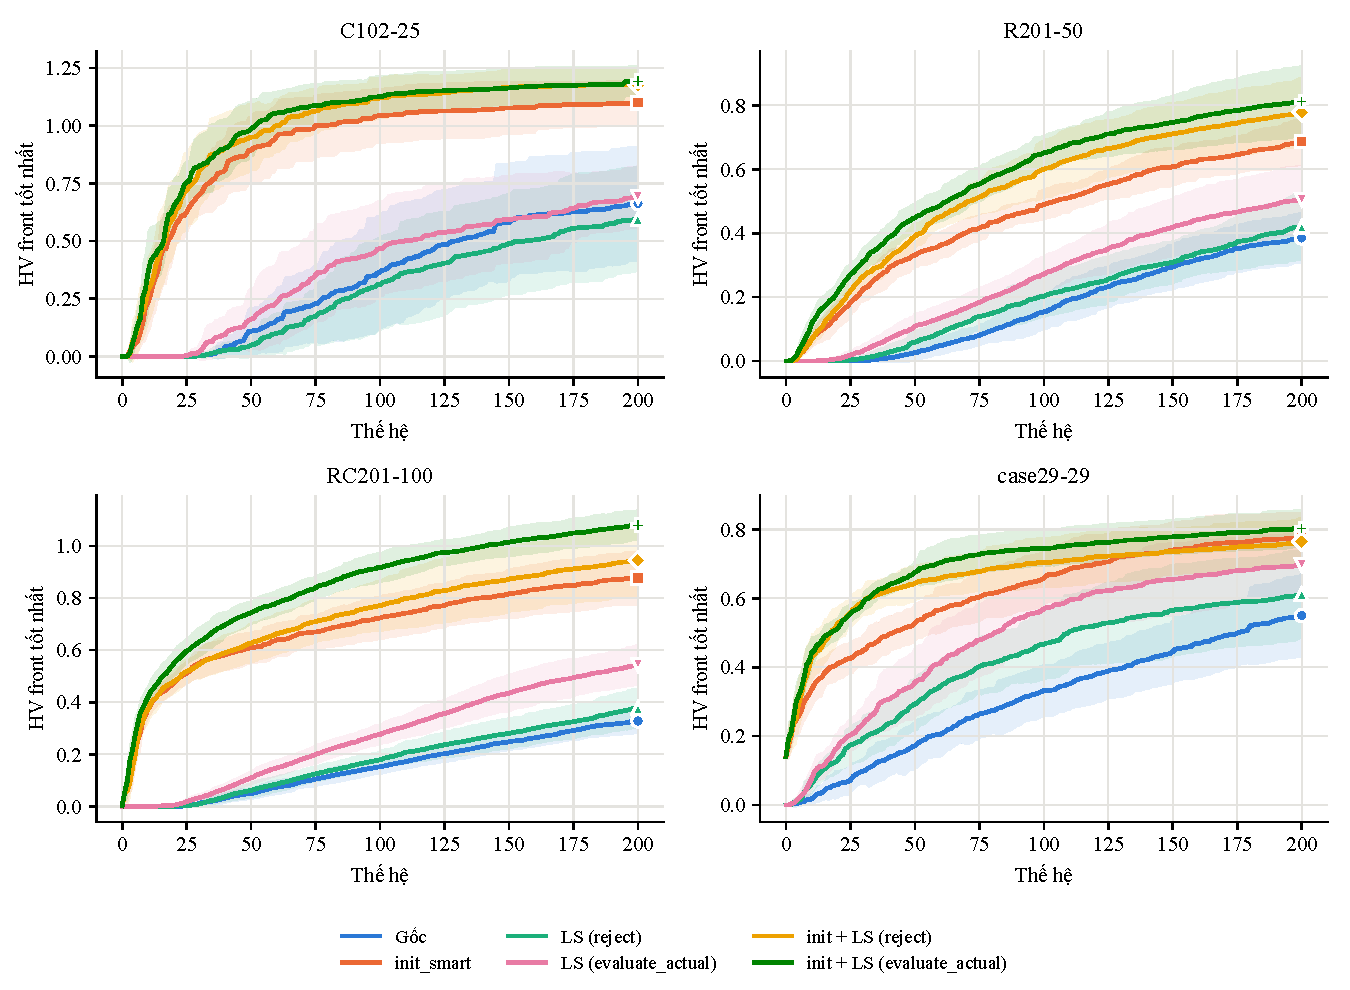
\includegraphics[width=\textwidth]{hoi_tu_hv.pdf}
\caption{HV của front tốt nhất theo thế hệ, trung bình $\pm$ độ lệch chuẩn qua 10 seed}
\label{fig:hoitu}
\end{figure}

Hình~\ref{fig:hoitu} cho thấy hai nhóm đường tách bạch. Các cấu hình có \code{init\_smart} có HV dương
ngay từ những thế hệ đầu và tăng nhanh trong khoảng 25 thế hệ đầu. Trên ba instance Solomon, các cấu
hình bắt đầu từ quần thể ngẫu nhiên có HV trung bình bằng 0 trong 10 đến 28 thế hệ đầu, vì front lúc đó
nằm ngoài vùng chuẩn hoá chung (điều này đã được ghi trong README của nhóm và là bình thường); trên
case29-29, HV dương ngay từ thế hệ thứ nhất. Ở mọi instance, HV vẫn còn tăng ở thế hệ 200, tức
200 thế hệ chưa đủ để thuật toán hội tụ hẳn.

\begin{figure}[H]
\centering
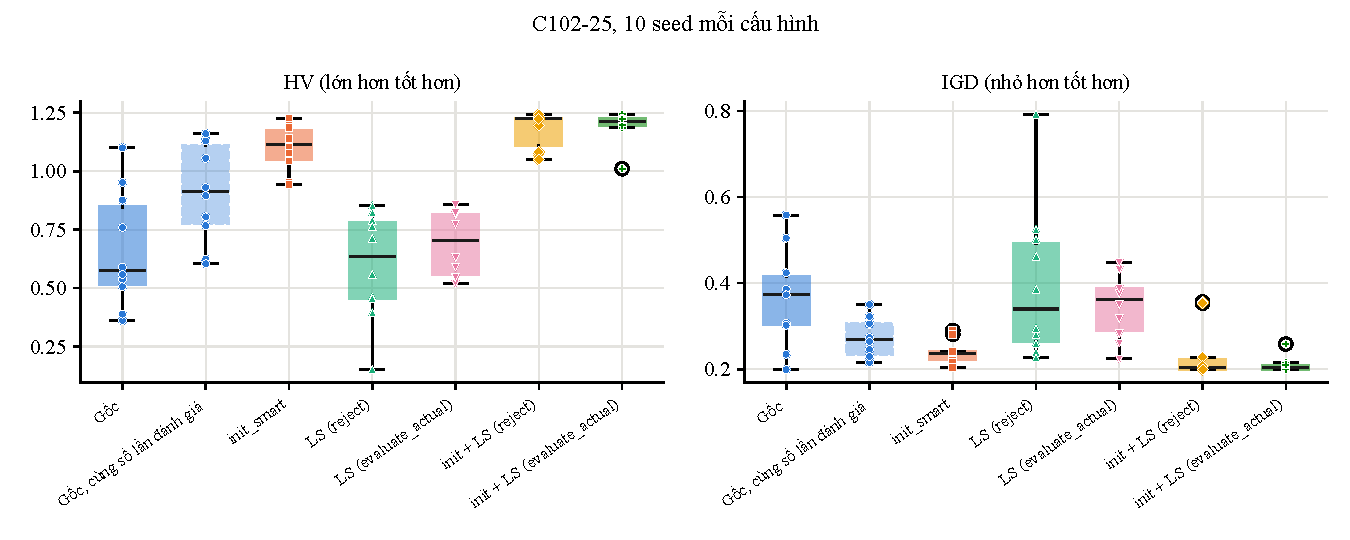
\includegraphics[width=\textwidth]{box_C102-25.pdf}\\[2pt]
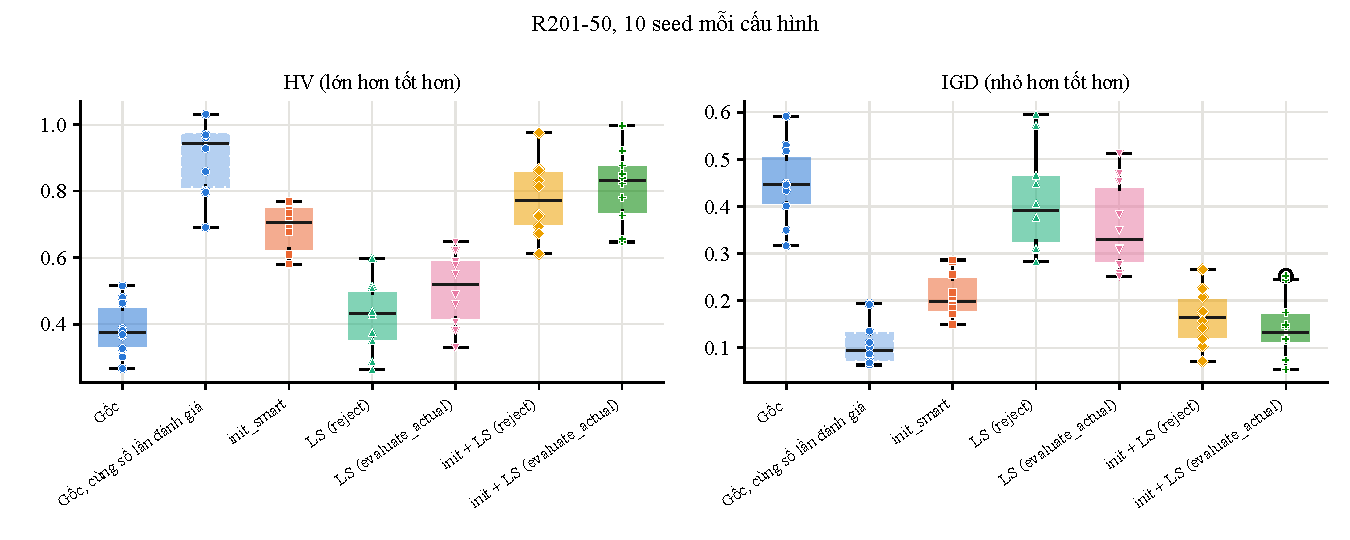
\includegraphics[width=\textwidth]{box_R201-50.pdf}
\caption{Phân bố HV và IGD qua 10 seed trên C102-25 và R201-50}
\label{fig:box1}
\end{figure}

\begin{figure}[H]
\centering
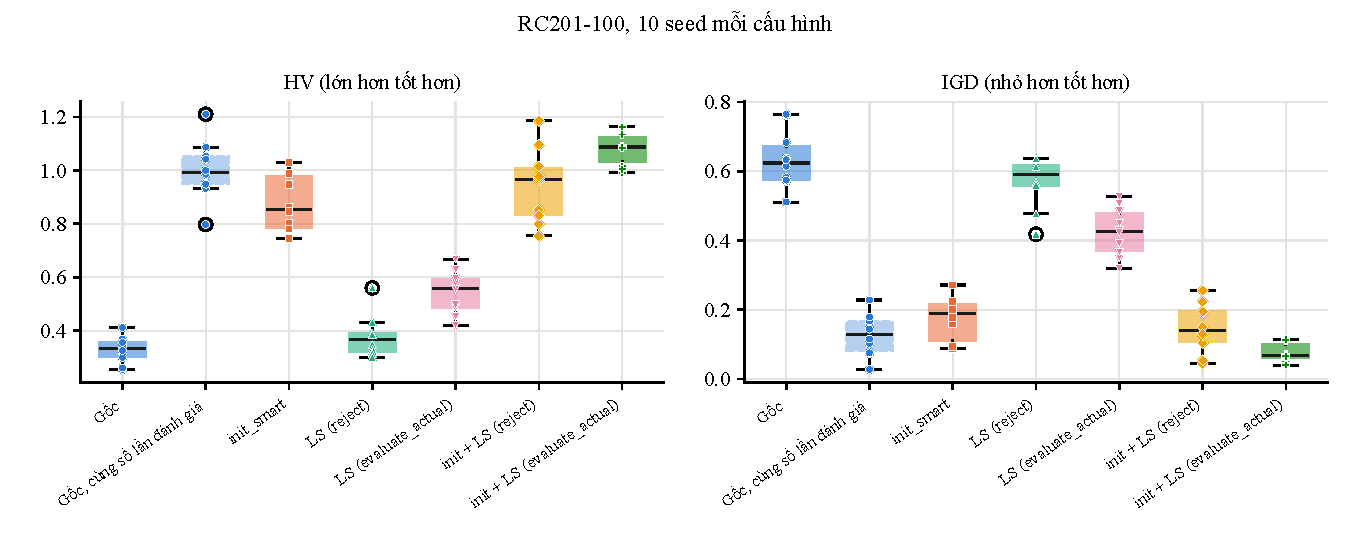
\includegraphics[width=\textwidth]{box_RC201-100.pdf}\\[2pt]
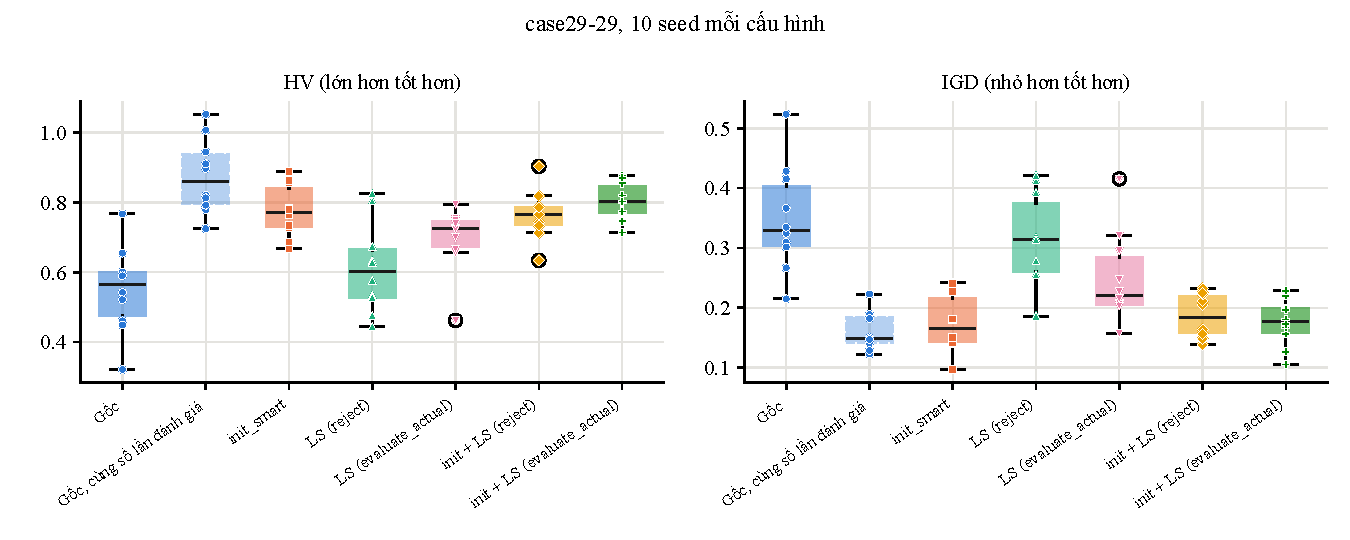
\includegraphics[width=\textwidth]{box_case29-29.pdf}
\caption{Phân bố HV và IGD qua 10 seed trên RC201-100 và case29-29}
\label{fig:box2}
\end{figure}

Biểu đồ hộp ở hình~\ref{fig:box1} và~\ref{fig:box2} xác nhận các nhận xét ở trên: hộp của các cấu hình có
\code{init\_smart} nằm cao hơn và hẹp hơn hộp của thuật toán gốc 200 thế hệ; hộp của thuật toán gốc chạy
dài (viền nét đứt) nằm cùng mức với các cấu hình kết hợp trên R201-50 và case29-29.

\begin{figure}[H]
\centering
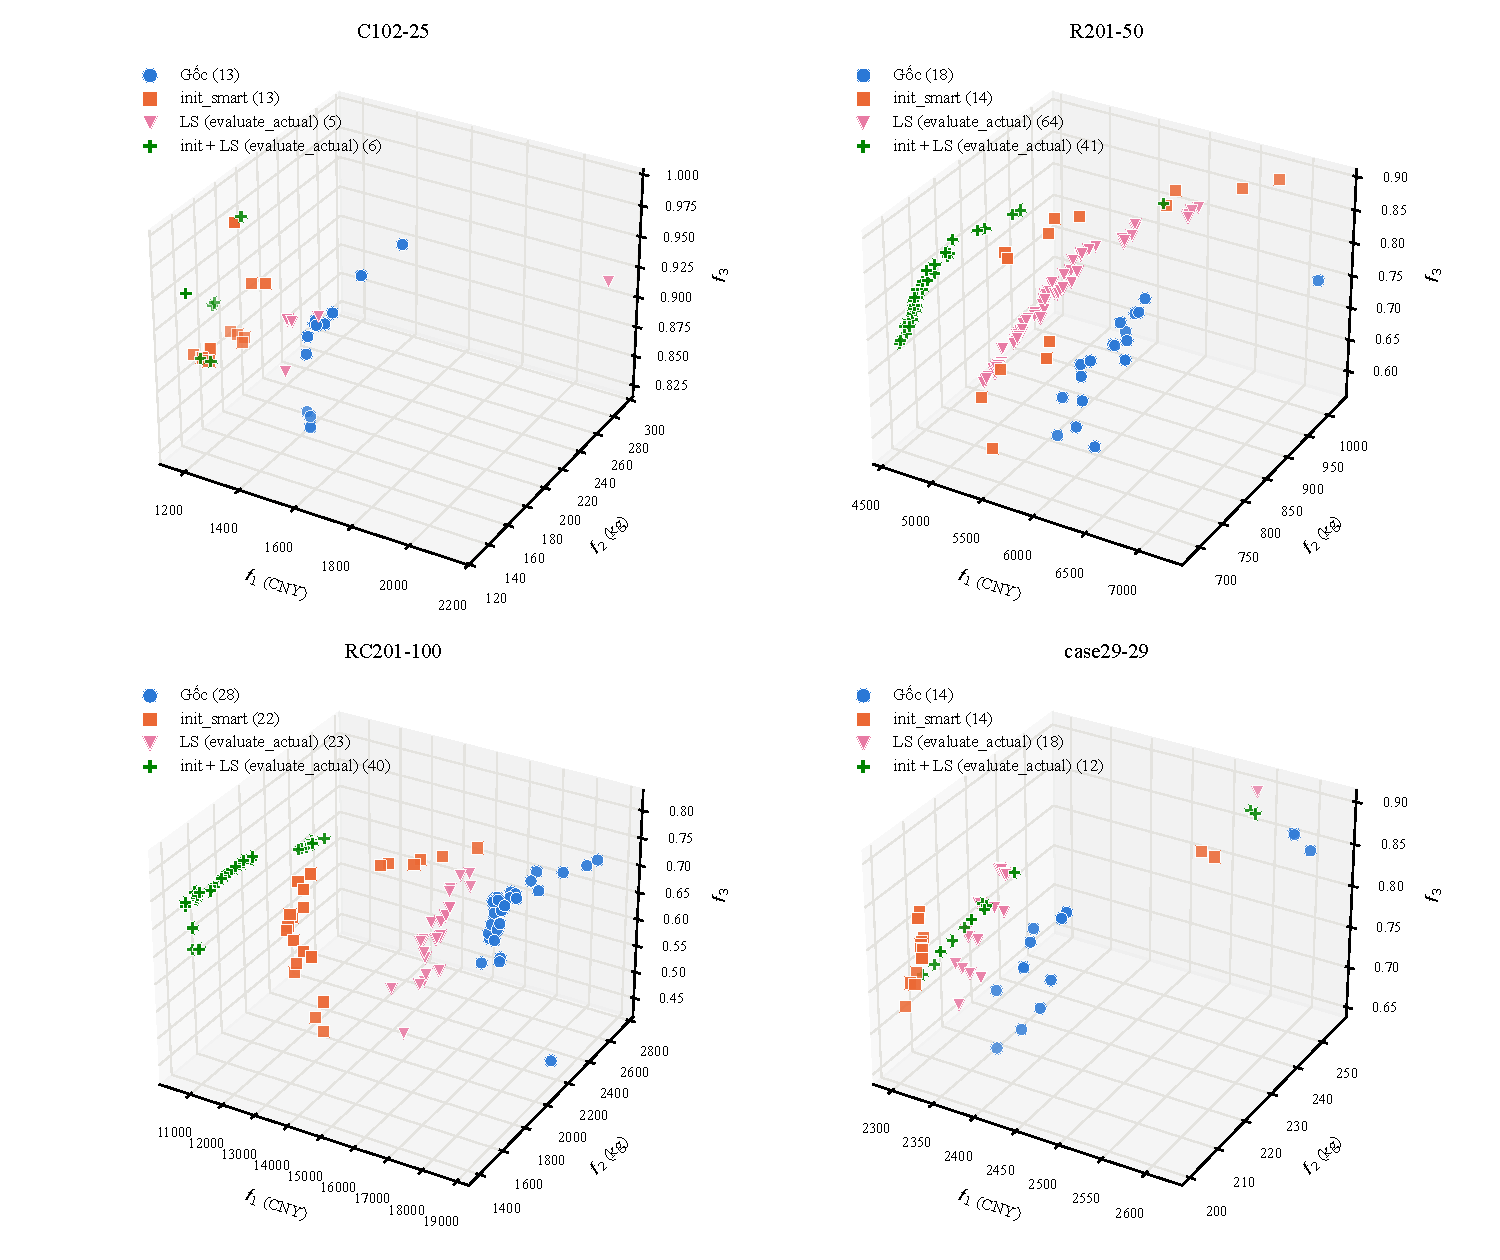
\includegraphics[width=\textwidth]{pareto_3d.pdf}
\caption{Front cuối không bị trội với seed 0, đơn vị gốc ($f_1$, $f_2$ cực tiểu, $f_3$ cực đại; số trong
ngoặc là số điểm trên front)}
\label{fig:pareto}
\end{figure}

Hình~\ref{fig:pareto} vẽ front cuối của bốn cấu hình với seed 0. Front của các cấu hình có khởi tạo thông
minh nằm ở vùng chi phí và khí thải thấp hơn hẳn, nhất là trên RC201-100. Hệ số tương quan Pearson giữa
$f_1$ và $f_2$ trên front gộp 10 seed dao động từ $-0{,}03$ đến 0,96 tuỳ cấu hình và instance. Tương quan
cao khi $f_1$ chủ yếu đi theo quãng đường, vì $f_2$ tỉ lệ với quãng đường; tương quan thấp khi phần phạt
đến muộn $F_4$ chi phối $f_1$, đúng như nhóm đã nhận xét ở giai đoạn 1 với các instance 100 khách.

Về ràng buộc số xe, front cuối của mọi cấu hình, mọi seed trên cả bốn instance đều không vượt giới hạn số
xe. Trội có ràng buộc của thuật toán gốc loại các nghiệm vượt giới hạn, và tìm kiếm cục bộ không làm nghiệm
hợp lệ trở thành không hợp lệ.

\section{Thảo luận}

\paragraph{Khởi tạo thông minh.} Đây là cải tiến có lợi rõ nhất: tốt hơn thuật toán gốc ở cả bốn instance,
không tốn thêm lần đánh giá, kết quả ổn định hơn giữa các seed. Hai heuristic bổ sung cho nhau: NN gieo
điểm ở vùng chi phí thấp, TW gieo điểm ở vùng hài lòng cao. Hạn chế là lợi thế giảm dần khi thuật toán
được chạy lâu hơn.

\paragraph{Tìm kiếm cục bộ.} Cách cắt tuyến \code{capacity\_time} làm phần lớn bước đi trong một tuyến bị
lệch biên, nên phiên bản thuần trong tuyến (\code{reject}) lãng phí phần lớn ngân sách đánh giá và không
hiệu quả. Cho phép đánh giá bằng bộ tuyến thật (\code{evaluate\_actual}) khắc phục được một phần và đem
lại cải thiện có ý nghĩa trên các instance lớn. Tuy vậy, ở cùng số lần đánh giá, tìm kiếm cục bộ chỉ thắng
thuật toán gốc chạy dài khi đi cùng khởi tạo thông minh, và chỉ trên hai trong bốn instance.

\paragraph{Giới hạn của thực nghiệm.} Thực nghiệm dùng bốn instance và 10 seed; kết luận chưa được kiểm
chứng trên đủ chín instance Solomon của bài báo. Kiểm định rank-sum được thực hiện riêng cho từng cặp,
không hiệu chỉnh cho nhiều phép so sánh. Các seed được ghép cặp giữa các cấu hình nên kiểm định có dấu
hạng (signed-rank) có thể phù hợp hơn; việc chọn kiểm định chính thức thuộc phần việc của TV3.
